\chapter{Photon Identification Optimization}

Photon identification in ATLAS is carried out through applying cuts to 9 shower shape variables that explain the longitudinal and lateral showering development of electromagnetic interaction in the calorimeter. These include variables describing the leakage in the hadronic calorimeter ($R_{had}$, $R_{had_1}$), widths of energy depositions in the \gls{EM} calorimeter ($w_{\eta_2}$, $w_{s3}$), energy ratios of depositions in the \gls{EM} calorimeter ($R_{\eta}$, $R_{\phi}$, $F_{side}$), and the energy difference and ratios of the strips ($\Delta E$, $E_{ratio}$). Two sets of cuts are defined, corresponding to two working points, nominally the \textit{tight} and \textit{loose} menus.

A schematic of all these variables can be found in Figure \ref{fig:ss-vars-schematic}. Additionally, a table describing these variables can be found in Table \ref{tab:ss-vars-table}.

% todo: maybe describe these a bit better https://arxiv.org/pdf/1606.01813.pdf 

In order to account for detector segmentation and differences in upstream material, cuts on these variables are derived in bins of \abseta. The intervals are 0.0, 0.6, 0.8, 1.15, 1.37, 1.52, 1.81, 2.01, 2.37, with a bin defined between each step (e.g. $[0.0,0.6)$, $[0.6,0.8)$, etc.) except over $[1.37,1.52)$ where the transition crack between the \gls{EMB} and \gls{EMEC} lies. 

% todo: make sure inclusivity here is correct

\begin{figure}[!thp]
    \centering
    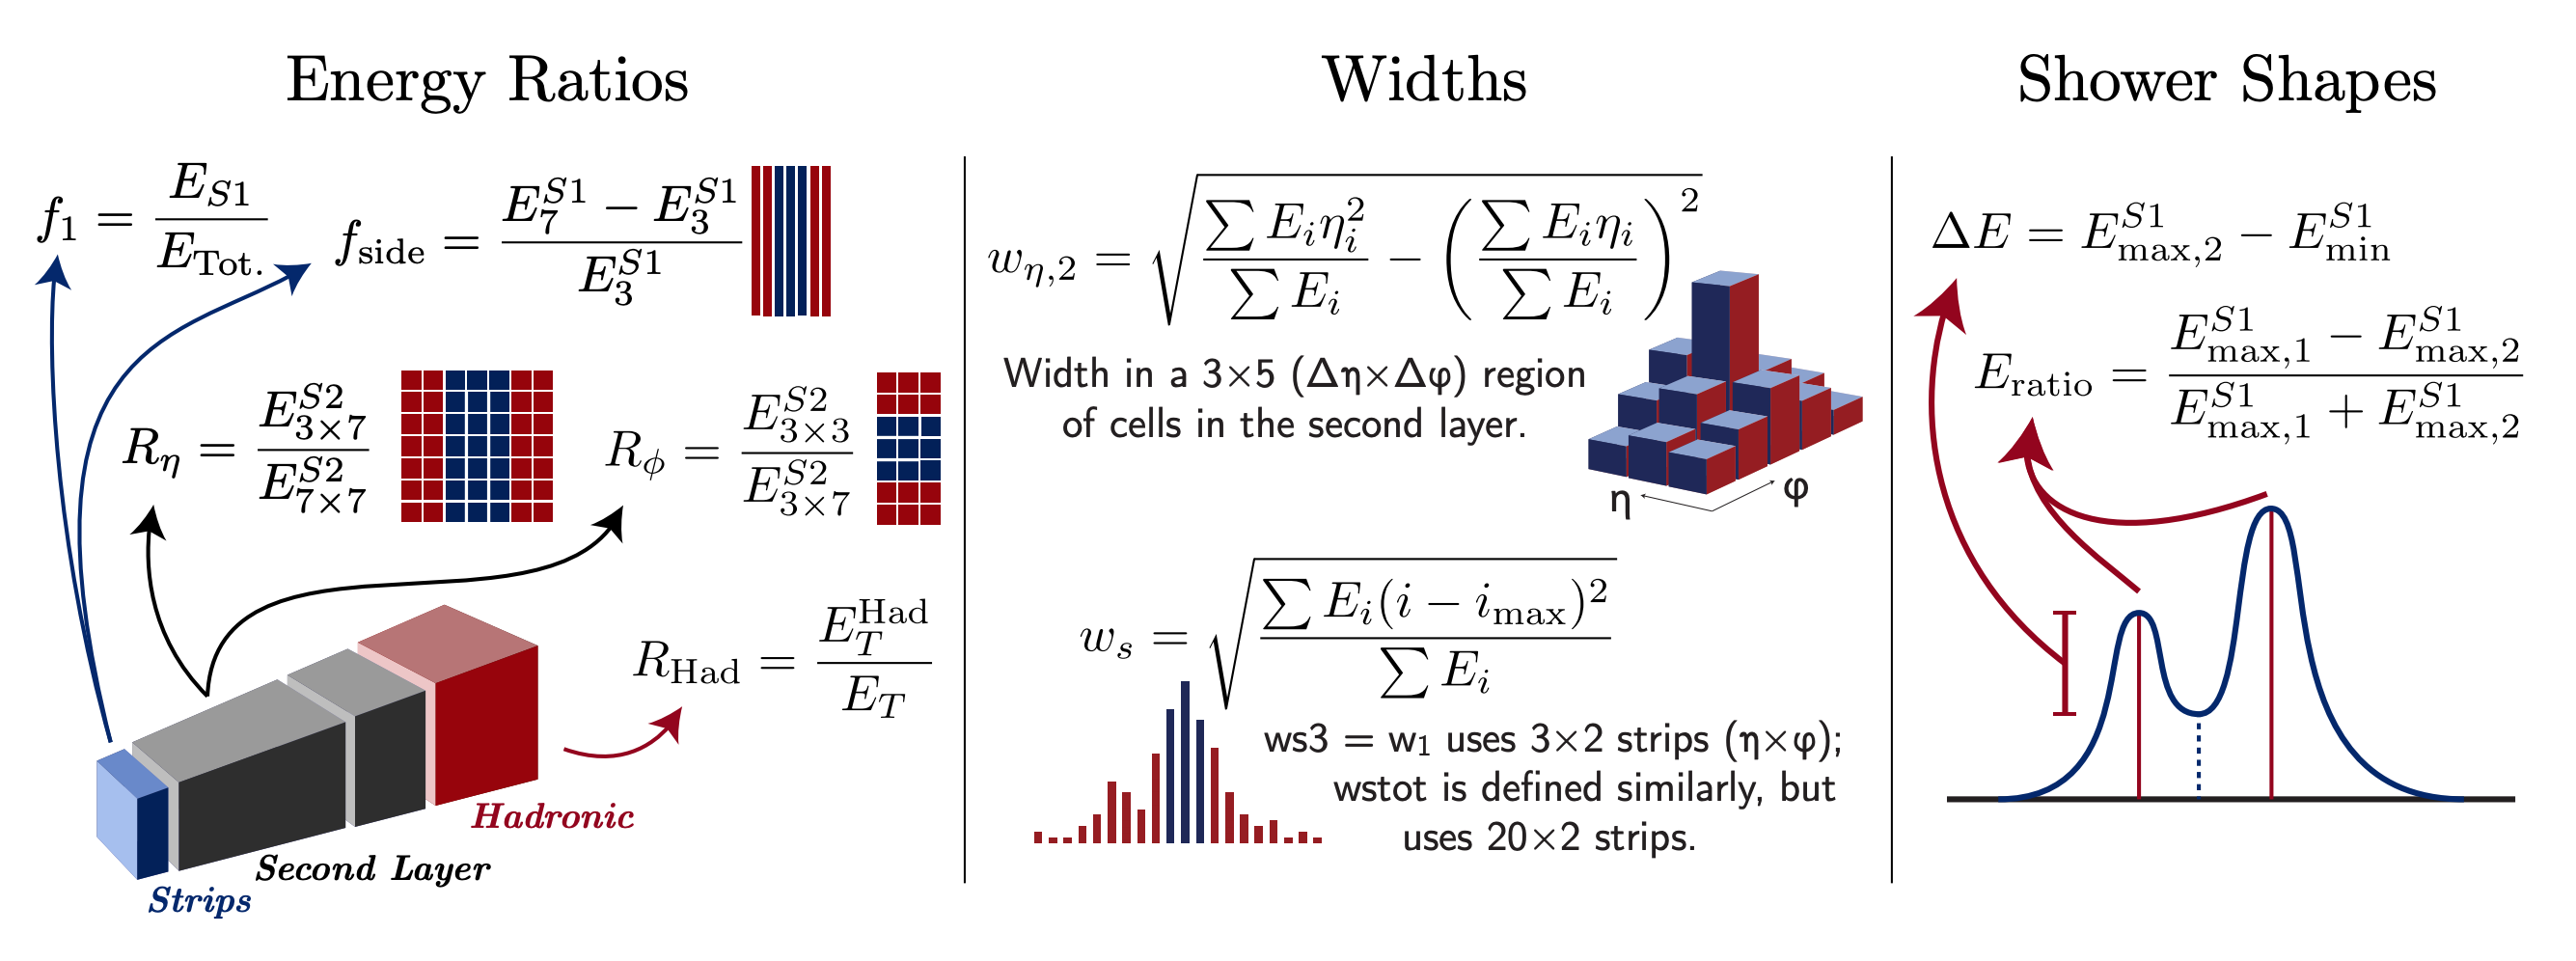
\includegraphics[width=.98\textwidth]{chapters/chapter4_photonID/images/ss-vars.png}
    \caption[Schematic of the shower shape variables used in the present cut-based photon identification menu.]
    {Schematic of the shower shape variables used in the present cut-based photon identification menu \cite{ss-var-schematic}.}
    \label{fig:ss-vars-schematic}
\end{figure}

\begin{table}[!thp]
    \centering
    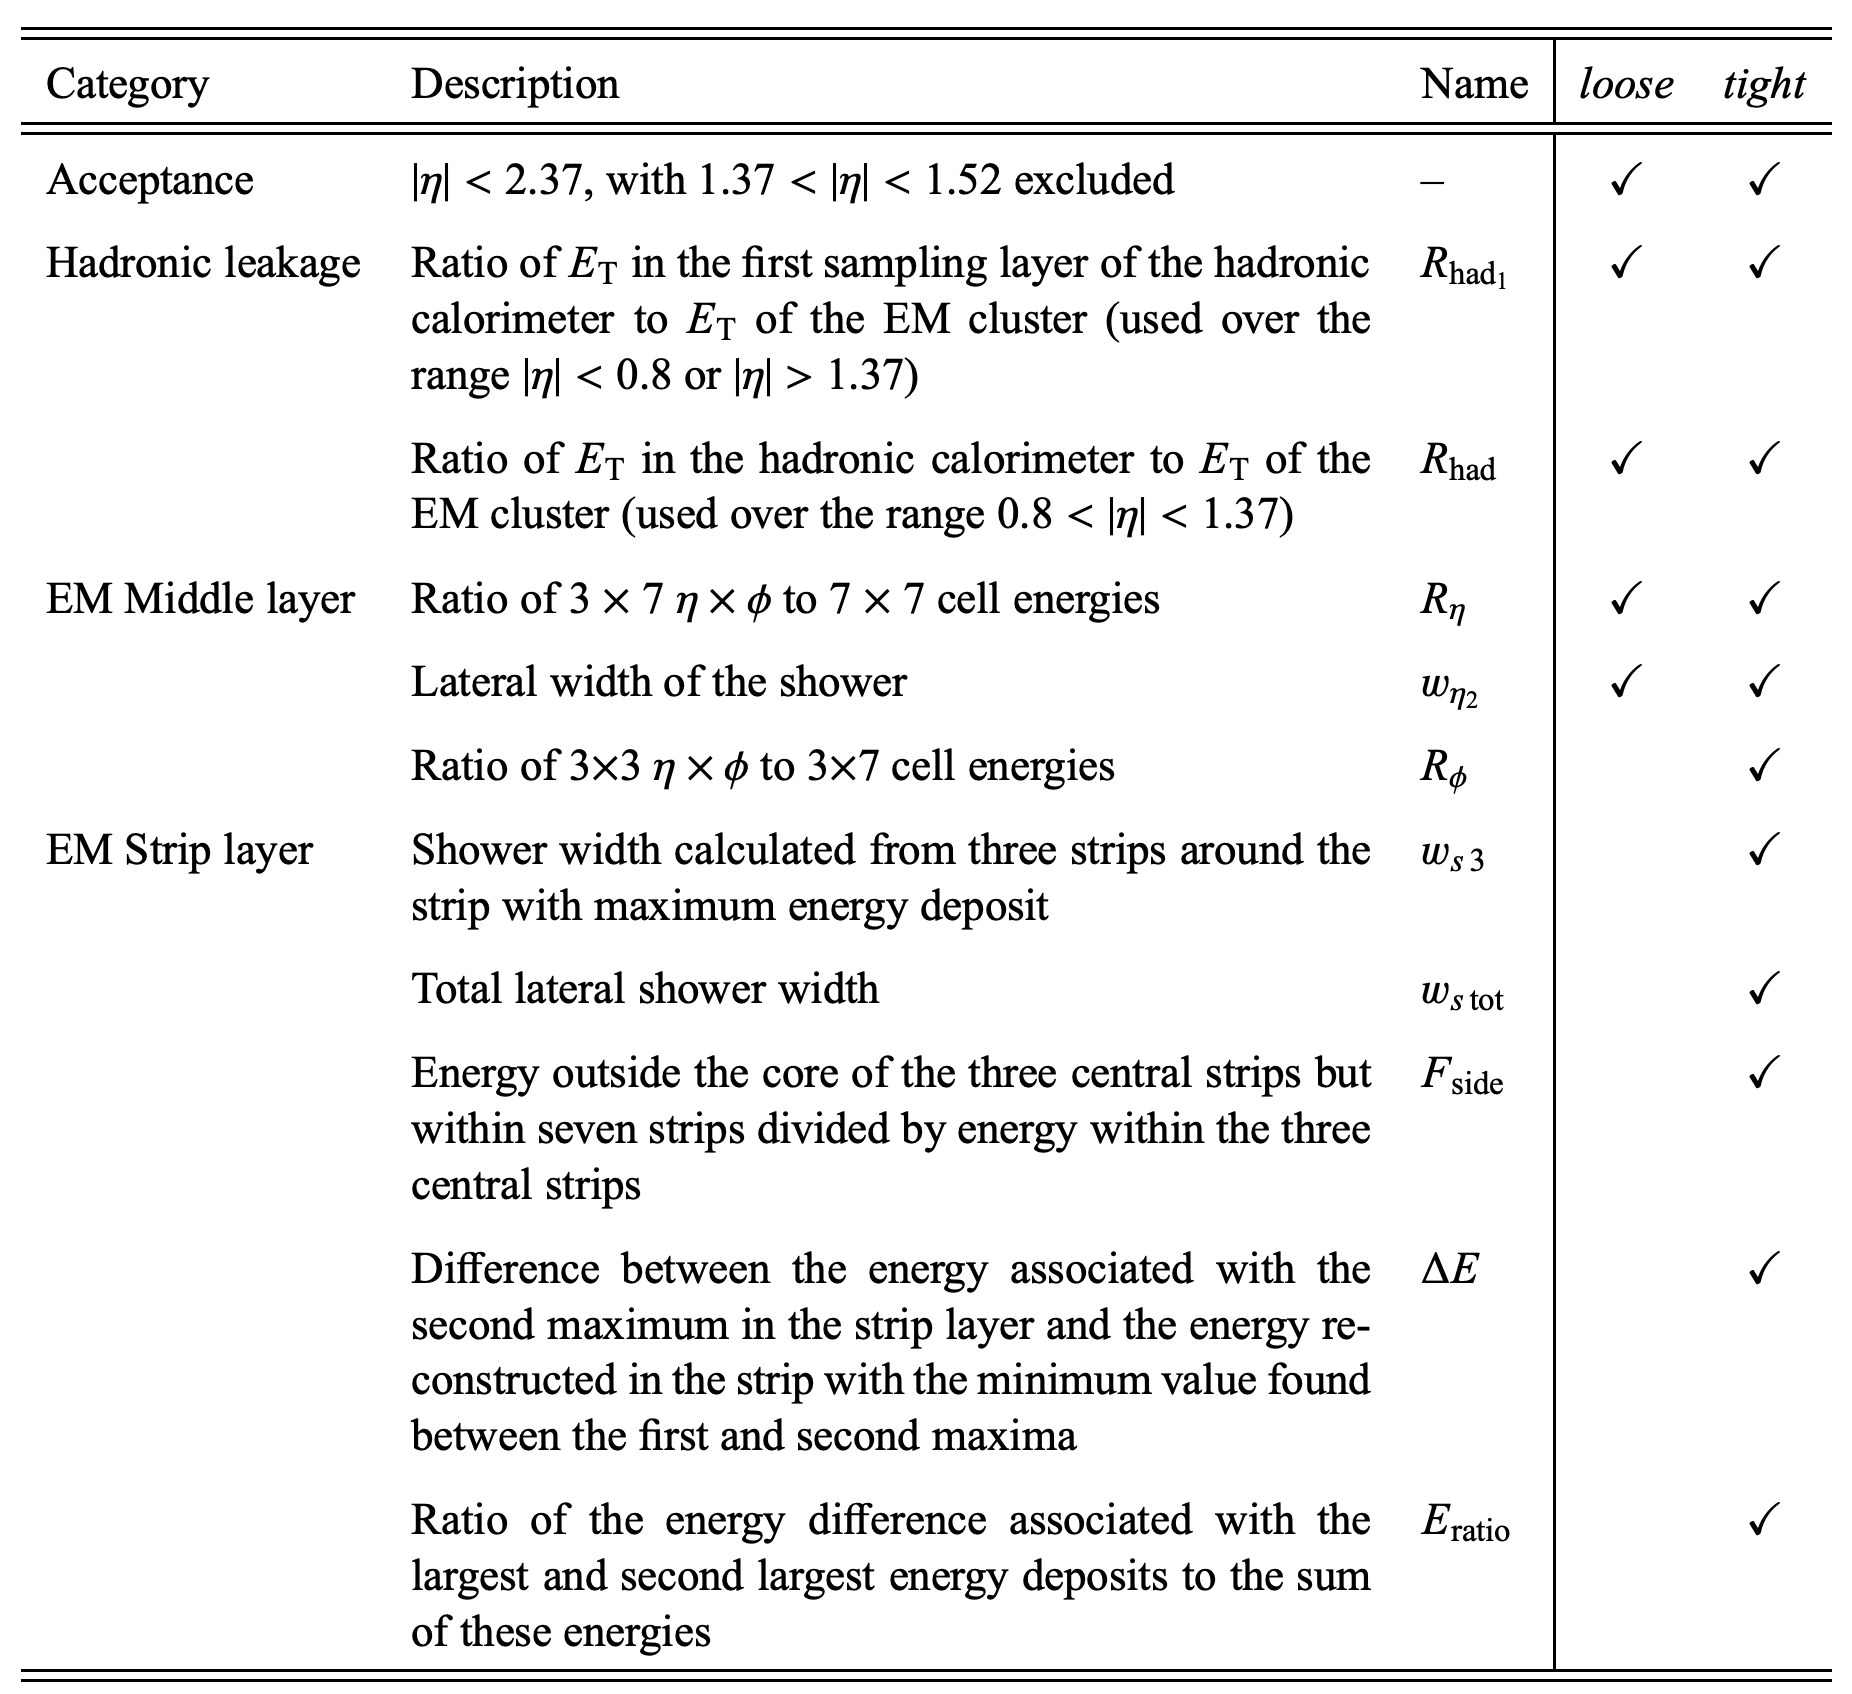
\includegraphics[width=.90\textwidth]{chapters/chapter4_photonID/images/ss-table.png}
    \caption[List of discriminating variables used in the present photon identification menu.]
    {List of discriminating variables used in the present photon identification menu \cite{r1-photonID}.}
    \label{tab:ss-vars-table}
\end{table}

\section{Samples} \label{sec:photon-id-samples}

In optimization of photon identification, the aim is to discriminate prompt photons from various background sources. The predominant background is that from hadronically decaying jets. 

For these studies, a sample of leading-order $\gamma+$jet events from $qg \rightarrow q \gamma$ and $q\bar{q} \rightarrow g \gamma$ hard scattering, as well as and quark fragmentation in QCD dijet events is used. Additionally, \gls{MC} truth information is used to require a prompt photon in the event. For background, a sample of all tree-level $2\rightarrow2$ QCD processes, except $\gamma+$jet events from quark fragmentation is used. \gls{MC} truth information is used to veto prompt photons in this sample as well. Both samples are generated using \PYTHIA. For both samples, simulation matched the detector conditions in the 2015 and 2016 data taking period. 



\section{Topological Clusters}

Photon reconstruction is performed through a method known as ``topological clustering,'' which is outlined in Section \ref{ssec:em-signatures}. In the calorimeter, energy depositions are clustered via this method, then merged into superclusters, which are ultimately the detector signature defined as the photon. The reconstructed observables of these topological clusters, or \textit{moments}, can be used to characterize them. This section will discuss the use of these topological cluster moments in photon identification to better reject background from non-prompt photons.

\noindent\textbf{Number of Topo-Clusters}\\
\indent As described in Section \ref{ssec:em-signatures}, photons are  superclusters, which can be made up of one or more topo-clusters as a result of cluster splitting or bremsstrahlung radiation. In over 90\% of photon events, there is only 1 topo-cluster associated to the photon supercluster. As a result, the quantities studied as inputs are all of the leading topo-cluster. Additionally, the number of topo-clusters is on average fewer for prompt photons than fakes, so this value is used as an input into the photon identification menu.

% TODO: Remake plot without name
\begin{figure}[!thp]
    \centering
    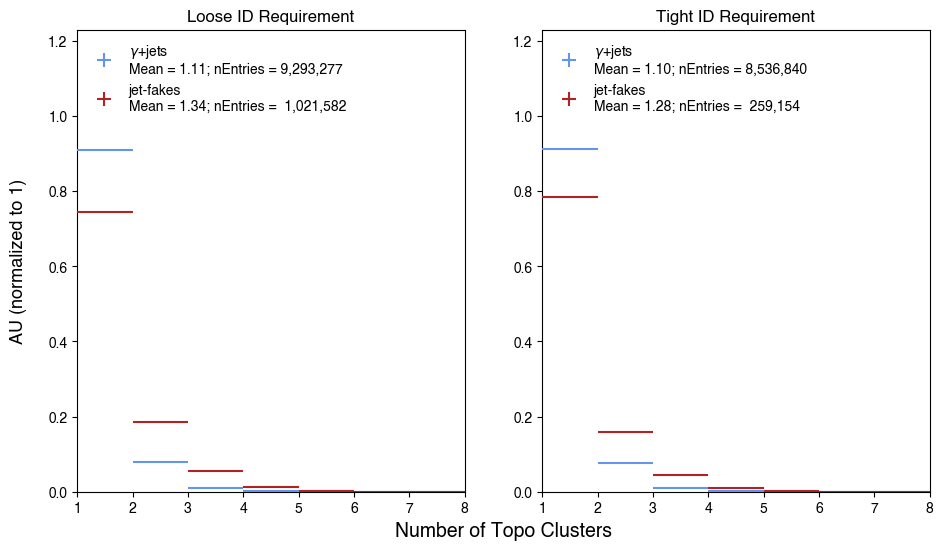
\includegraphics[width=.90\textwidth]{chapters/chapter4_photonID/images/hists/y_nTopoClusters.png}
    \caption[Number of topo-clusters in photon superclusters]
    {Number of topo-clusters in photon superclusters in truth-matched $\gamma+$jet events and truth-vetoed jet fake events} 
    \label{fig:topo-geom}
\end{figure}


\noindent\textbf{Shape Information}\\
\indent The size of the topological cell is parametrized by moments in $r_i$ and $\lambda_i$, which are defined as:

\begin{equation}
    r_i = |(\vec{x_i} - \vec{c}) \times \vec{s}| \text{\hspace{2em}(radial distance to shower axis)} \\
\end{equation}
\begin{equation}
    \lambda_i = (\vec{x_i} - \vec{c}) \cdot \vec{s} \text{\hspace{2em}(longitudinal distance to shower center of gravity)} 
\end{equation}

Where $\vec{s}$ is the shower axis and $\vec{c}$ is the center of gravity. Through this parametrization, the topo-cluster can be analyzed as a spheroid, with the second moments in $r$ and $\lambda$ as the extensions. $\sqrt{\langle \lambda^2 \rangle}$ is the semi-major axis in depth (along the shower axis), $\sqrt{\langle r^2 \rangle}$ is the semi-major axis in width. The distribution of these two parameters are shown for the leading topo cluster in Figures \ref{fig:topo-secondLambda} and \ref{fig:topo-secondR}, after applying the current loose and tight photon identification criteria.

\begin{figure}[!thp]
    \centering
    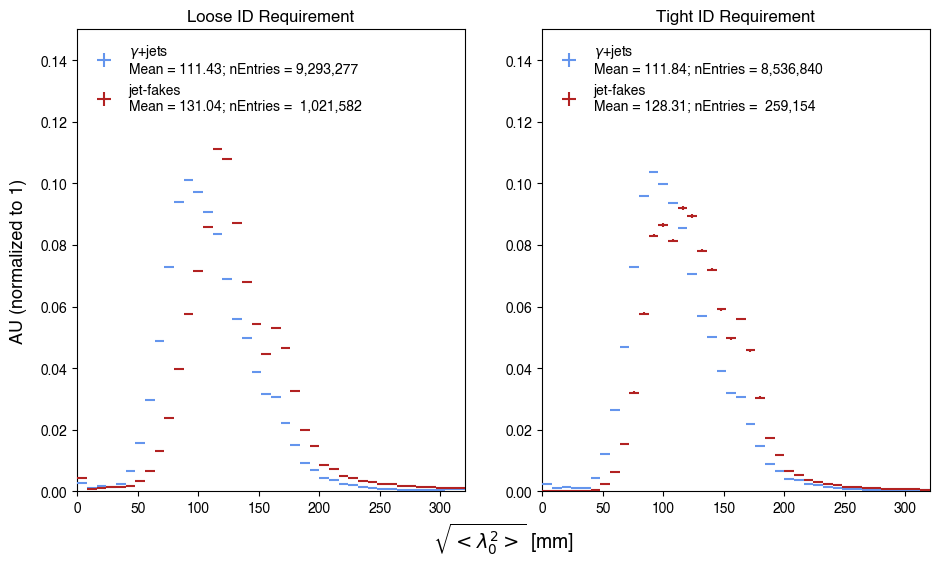
\includegraphics[width=.9\textwidth]{chapters/chapter4_photonID/images/hists/y_topoCluster0_secondLambda.png}
    \caption[The distribution of the semi-major axis in depth for the leading topo-cluster]{The distribution of the semi-major axis in depth for the leading topo-cluster in truth-matched $\gamma+$jet events and truth-vetoed jet fake events.}
    \label{fig:topo-secondLambda}

\end{figure}

\begin{figure}[!thp]
    \centering 
    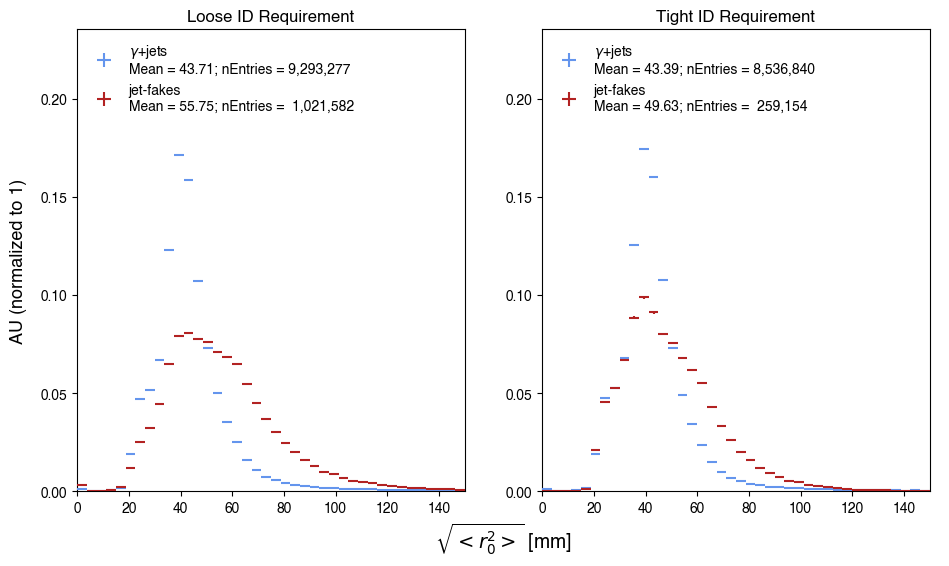
\includegraphics[width=.9\textwidth]{chapters/chapter4_photonID/images/hists/y_topoCluster0_secondR.png}
    \caption[The distribution of the semi-major axis in width for the leading topo-cluster]{The distribution of the semi-major axis in width for the leading topo-cluster in truth-matched $\gamma+$jet events and truth-vetoed jet fake events.}
    \label{fig:topo-secondR}
\end{figure}



\noindent\textbf{Location Information}\\
\indent The location of the topo-cluster is calculated from the first moments of the three cartesian coordinates, describing the position of $\vec{c}$. Due to azimuthal symmetry in the detector, the key component to locational parametrization of topo-clusters is the depth in the calorimeter. Thus, this location can be described via $\lambda_{clus}$, the distance of the center of gravity from the front face of the calorimeter. This distribution is shown in Figure \ref{fig:topo-centerLambda}.

\begin{figure}[!thp]
    \centering 
    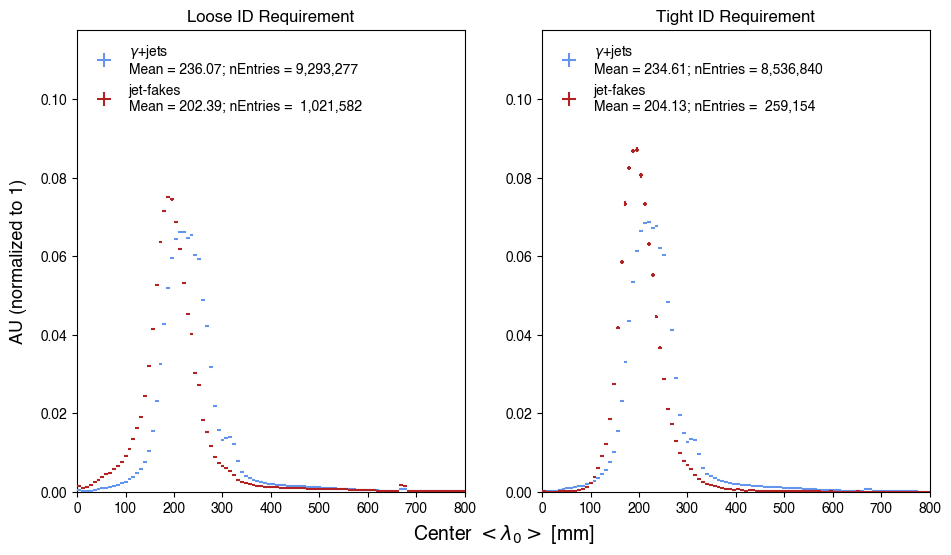
\includegraphics[width=.9\textwidth]{chapters/chapter4_photonID/images/hists/y_topoCluster0_centerLambda.png}
    \caption[The distribution of the centroid depth ($<\lambda_{0}>$) of the leading topo-cluster]{The distribution of the centroid depth ($<\lambda_{0}>$) of the leading topo-cluster in truth-matched $\gamma+$jet events and truth-vetoed jet fake events.}
    \label{fig:topo-centerLambda}
\end{figure}

A visualization of the geometric moments, both location and shape can be found in Figure \ref{fig:topo-geom}, with relevant spacial parameters (i.e. $\vec{c}$, $\vec{s}$, etc) shown and defined.

\begin{figure}[!thp]
    \centering
    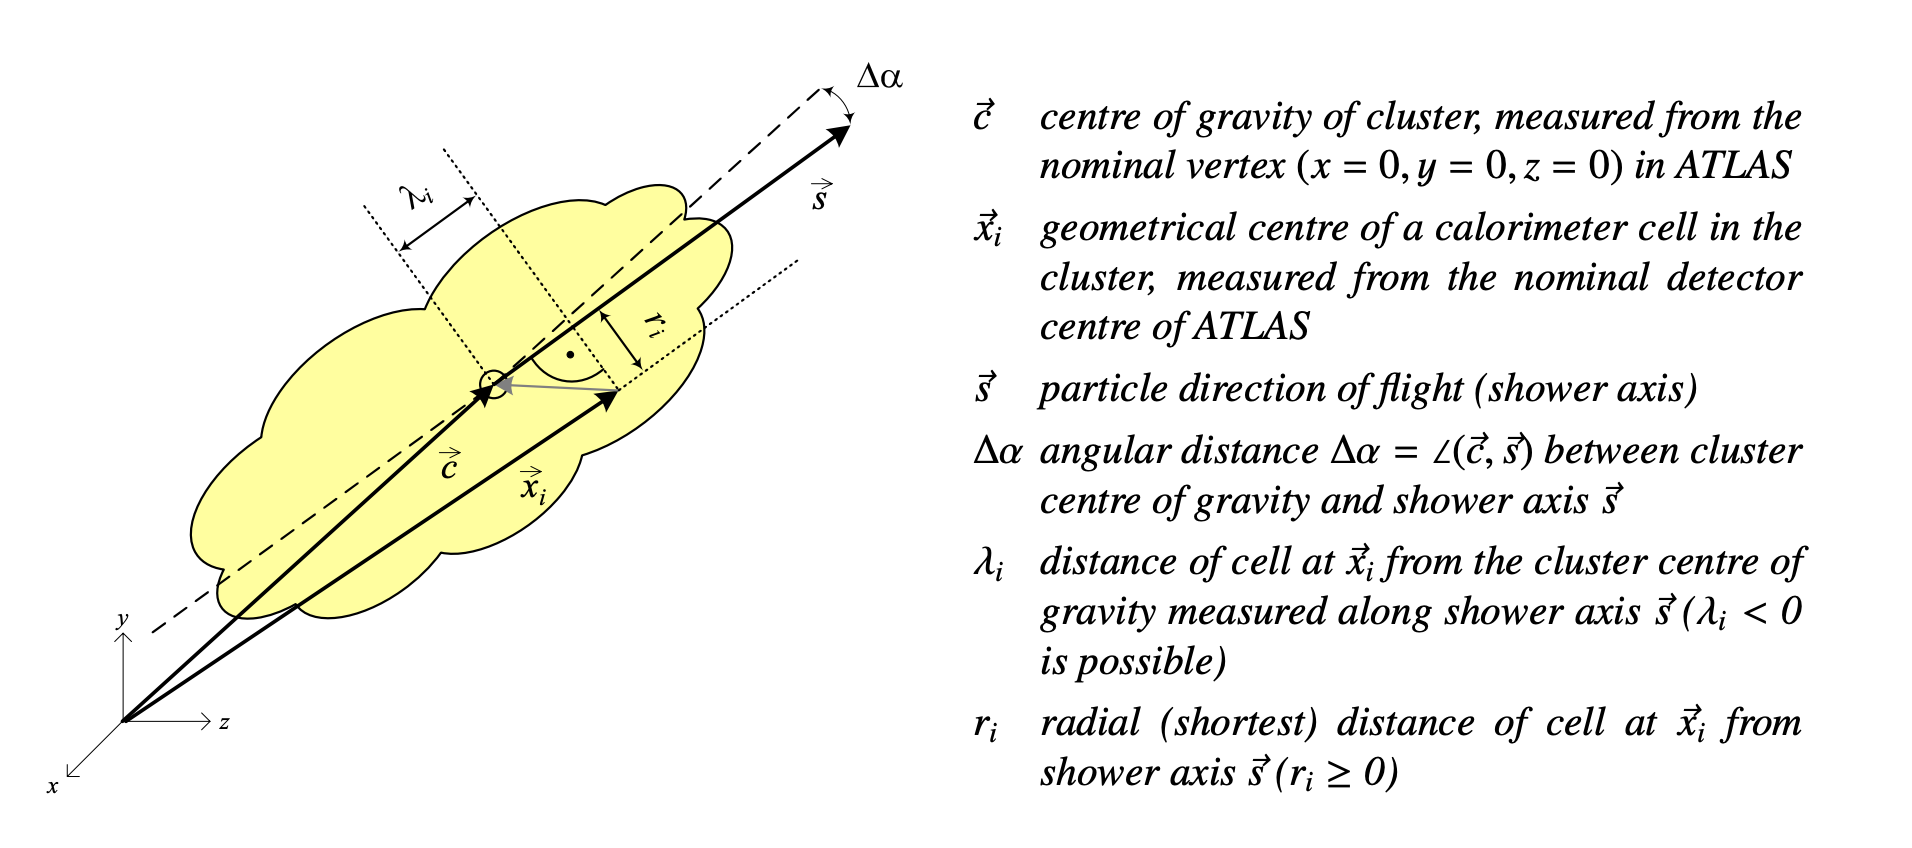
\includegraphics[width=.90\textwidth]{chapters/chapter4_photonID/images/geom-moments.png}

    \caption[The geometric moments and relevant parameters for topo-clusters.]
    {The geometric moments and relevant parameters for topo-clusters \cite{topo-clustering-r1}.}
    \label{fig:topo-geom}
\end{figure}


\noindent\textbf{Additional Moments}\\
\indent Beyond the shape and location information, there are several other moments that can be used. Two are considered as inputs into the photon identification menu, cluster isolation and \gls{EM} probability.

The signal thresholds built into the topological clustering algorithm are constructed to suppress noise, but lead to signal losses at the perimeter of clusters. The isolation moment, $f_{\text{iso}}$, measures the degree of isolation of a cluster. It is constructed as a weighted fraction of the sampling layer energy ($E_{s}^{\text{EM}}$) of non-clustered neighbor cells on the perimeter of the topo-cluster in the sampling layer. It is given by

\begin{equation}
    f_{\text{iso}} = \frac
    {
    \sum_{S \in \{ \text{samplings with} E_{s}^{\text{EM}} > 0 \} }  
    E_{s}^{\text{EM}} N_{\text{cell},s}^{\text{noclus}} / N_{\text{cell},s}^{\text{neighbor}}
    } 
    {
        \sum_{S \in \{ \text{samplings with} E_{s}^{\text{EM}} > 0 \} }
    }.
\end{equation}

Here, $N_{\text{cell},s}^{\text{noclus}} / N_{\text{cell},s}^{\text{neighbor}}$ is the ratio of unclustered perimeter cells to the total number of perimeter cells for a given cluster. This is summed across all sampling layers with positive energy, $s$. For the signal and background samples, the isolation is shown using the existing loose and tight identification criteria in Figure \ref{fig:topo-isolation}.

\begin{figure}[!thp]
    \centering 
    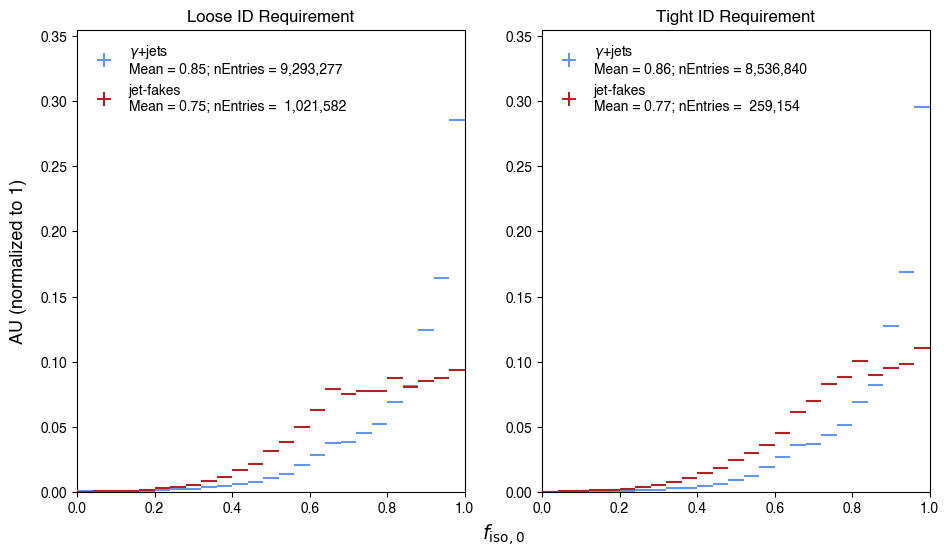
\includegraphics[width=.9\textwidth]{chapters/chapter4_photonID/images/hists/y_topoCluster0_isolation.png}
    \caption[The distribution of the isolation moment of the leading topo-cluster]{The distribution of the isolation moment of the leading topo-cluster in truth-matched $\gamma+$jet events and truth-vetoed jet fake events}
    \label{fig:topo-isolation}
\end{figure}

Energy losses in topo-clusters are corrected through a method known as \glsfirst{LCW} calibration. Since energy losses differ between hadronic and electromagnetic deposits, the \gls{LCW} calibration includes a step where the probability that a topo-cluster originates from an electromagnetic shower is evaluated.

The likelihood is defined through measuring the efficiency for detecting an EM-like cluster in bins of four other topo-cluster observables, defined by

\begin{equation}
    \mathfrak{O}_{\text{clus}}^{\text{class}} = \{
        E_{\text{clus}}^{\text{EM}},
        \eta_{\text{clus}},
        \log_{10}(\rho_{\text{clus}} / \rho_{\text{0}}) - \log_{10}(E_{\text{clus}}^{\text{EM}} / E_{\text{0}}),
        \log_{10}(\lambda_{\text{clus}} / \lambda_{\text{0}}
    \}
\end{equation}

where $\rho_0 = 1$ MeV mm$^-3$, $E_0 = \unit{1}{\MeV}$, $\lambda_{0} = \unit{1}{\mm}$. These bins (denoted $ijkl$) can then be used to define the likelihood, $ \mathcal{P}_{\text{clus}}^{\text{EM}}$, in each bin as


\begin{equation}
    \mathcal{P}_{\text{clus}}^{\text{EM}} ( E_{\text{clus}}^{\text{EM}}, \eta_{\text{clus}}, \rho_{\text{clus}} / E_{\text{clus}}^{\text{EM}}, \lambda_{\text{clus}}) \mapsto \mathcal{P}_{\text{clus}, ijkl}^{\text{EM}}  = \frac{\epsilon^{\pi^0}_{ijkl}}{ \epsilon^{\pi^0}_{ijkl} + 2\epsilon^{\pi^\pm}_{ijkl}}
\end{equation}


Where $\epsilon^{\pi^0(\pi^\pm)}_{ijkl}$ is the efficiency, defined as
\begin{equation}
    \epsilon^{\pi^0(\pi^\pm)}_{ijkl} = \frac{ N^{\pi^0(\pi^\pm)}_{ijkl} }{N^{\pi^0(\pi^\pm)}_{ij}}
\end{equation}

For $N^{\pi^0(\pi^\pm)}_{ijkl}$ topo-clusters in a given bin $ijkl$ and $N^{\pi^0(\pi^\pm)}_{ij}$ topo-clusters in bin $ij$ of the $(E_{\text{clus}}^{\text{EM}}, \eta_{\text{clus}})$ phase space. This likelihood, $\mathcal{P}_{\text{clus}}^{\text{EM}}$, by definition is bounded from 0 to 1, and considered as an input into the photon ID menu. This distribution is shown in Figure \ref{fig:topo-emProb}, with both the current loose and tight photon identification criteria applied.

\begin{figure}[!thp]
    \centering 
    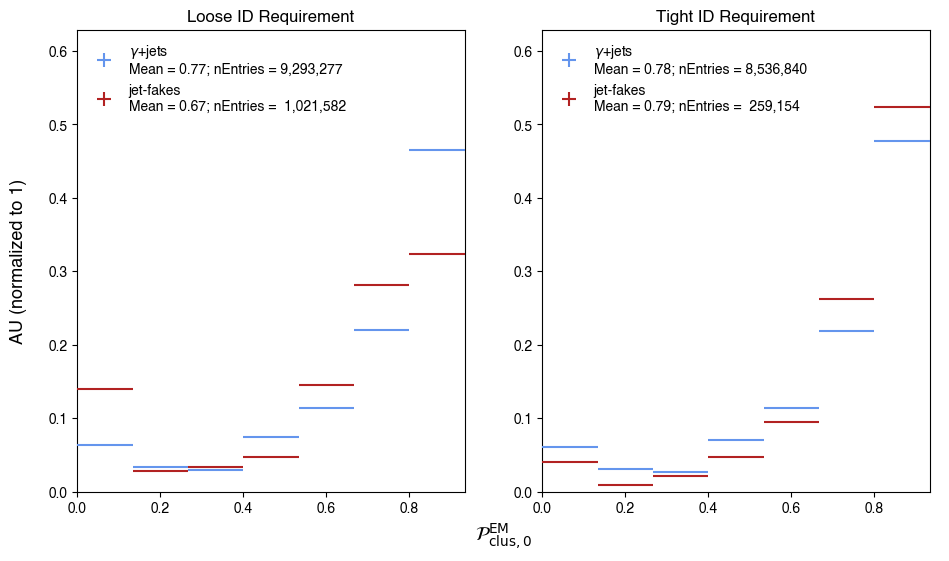
\includegraphics[width=.9\textwidth]{chapters/chapter4_photonID/images/hists/y_topoCluster0_emProbability.png}
    \caption[The distribution of the \gls{EM} probability moment of the leading topo-cluster]{The distribution of the \gls{EM} probability moment of the leading topo-cluster in truth-matched $\gamma+$jet events and truth-vetoed jet fake events}
    \label{fig:topo-emProb}
\end{figure}


\subsection{Data-MC Comparison}
In order to ensure that the topological clusters are properly modeled in the \gls{MC}, the variables investigated are compared to data. To do so, the present tight photon ID is applied to both the \gls{MC} and data. Furthermore, photons in \gls{MC} must correspond to a truth photon. 


This section includes the comparisons for unconverted photons which are considered for adding to the photon ID menu. Converted comparisons will be included into Appendix 

% TODO: add appendix

%todo: add plots

\begin{figure}[!thp]
    \centering
    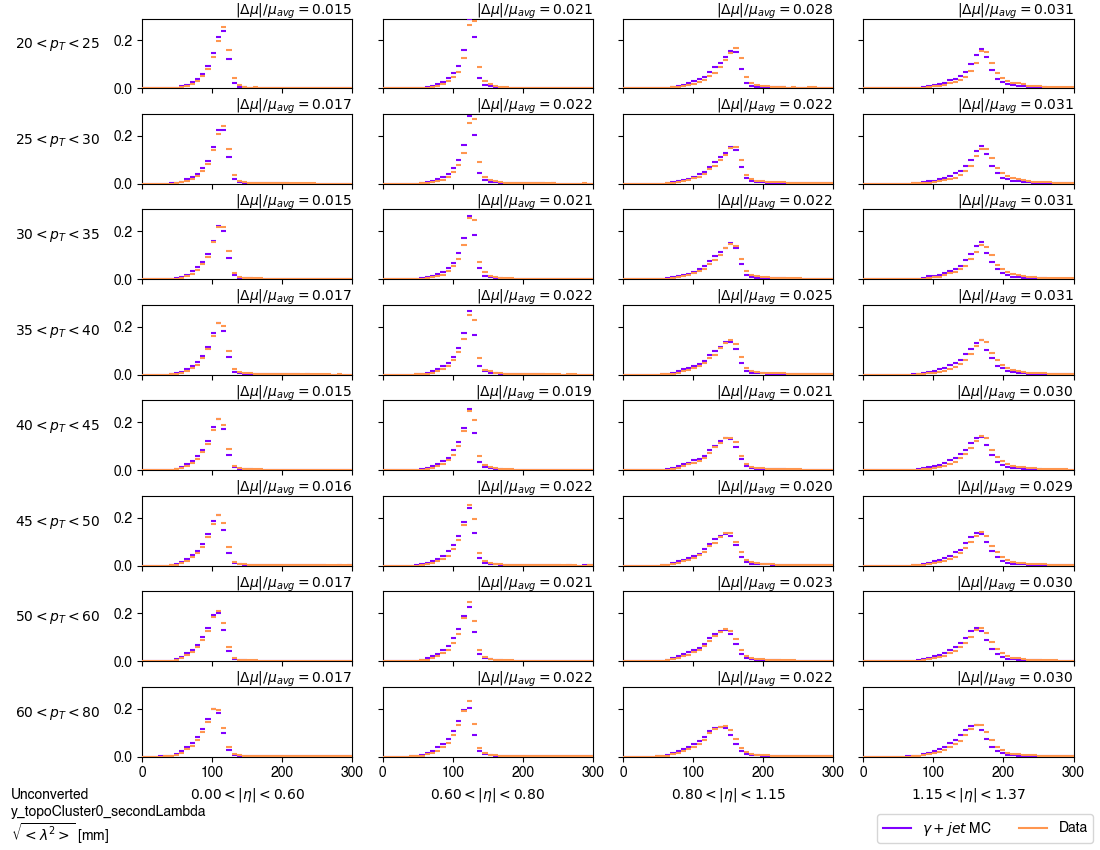
\includegraphics[width=.80\textwidth]{chapters/chapter4_photonID/images/y_topoCluster0_secondLambda_Unconverted_lowerEta.png}
    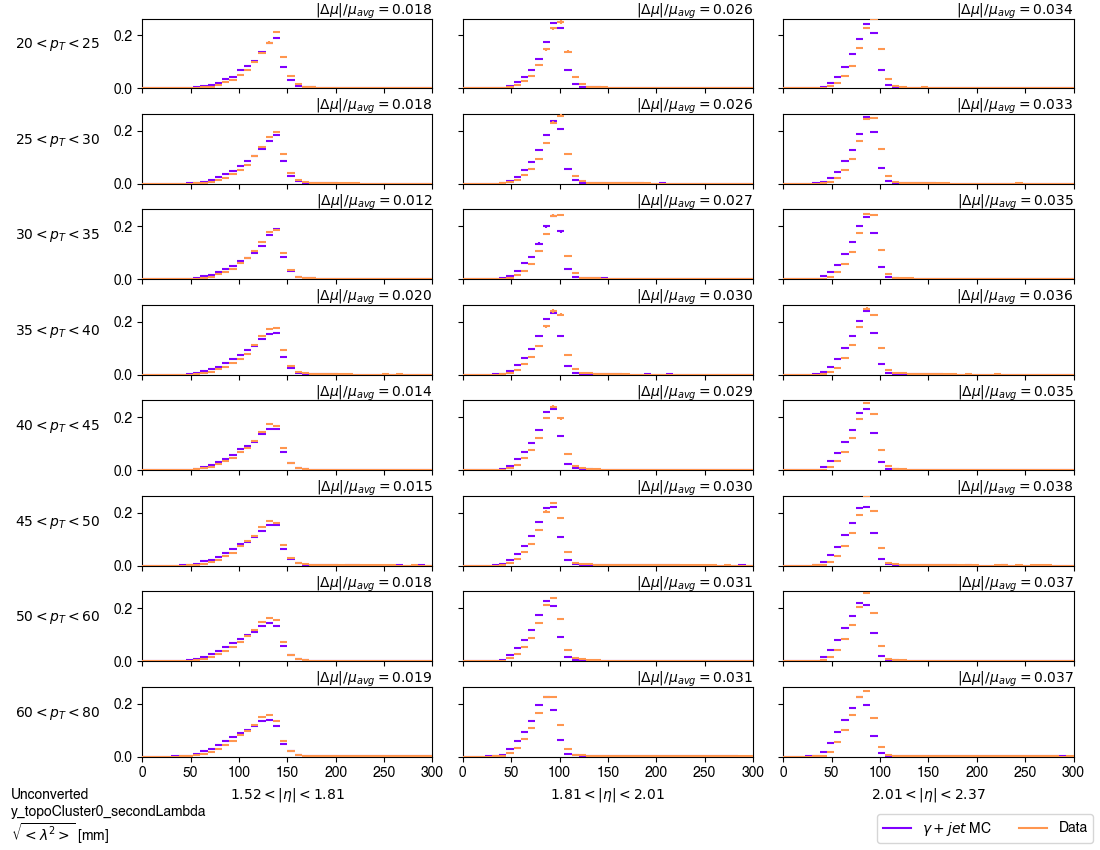
\includegraphics[width=.80\textwidth]{chapters/chapter4_photonID/images/y_topoCluster0_secondLambda_Unconverted_upperEta.png}
    \caption{Data-MC comparison for the semi-major axis in depth ($\sqrt{\lambda^2}$).}
\end{figure}
\begin{figure}[!thp]
    \centering
    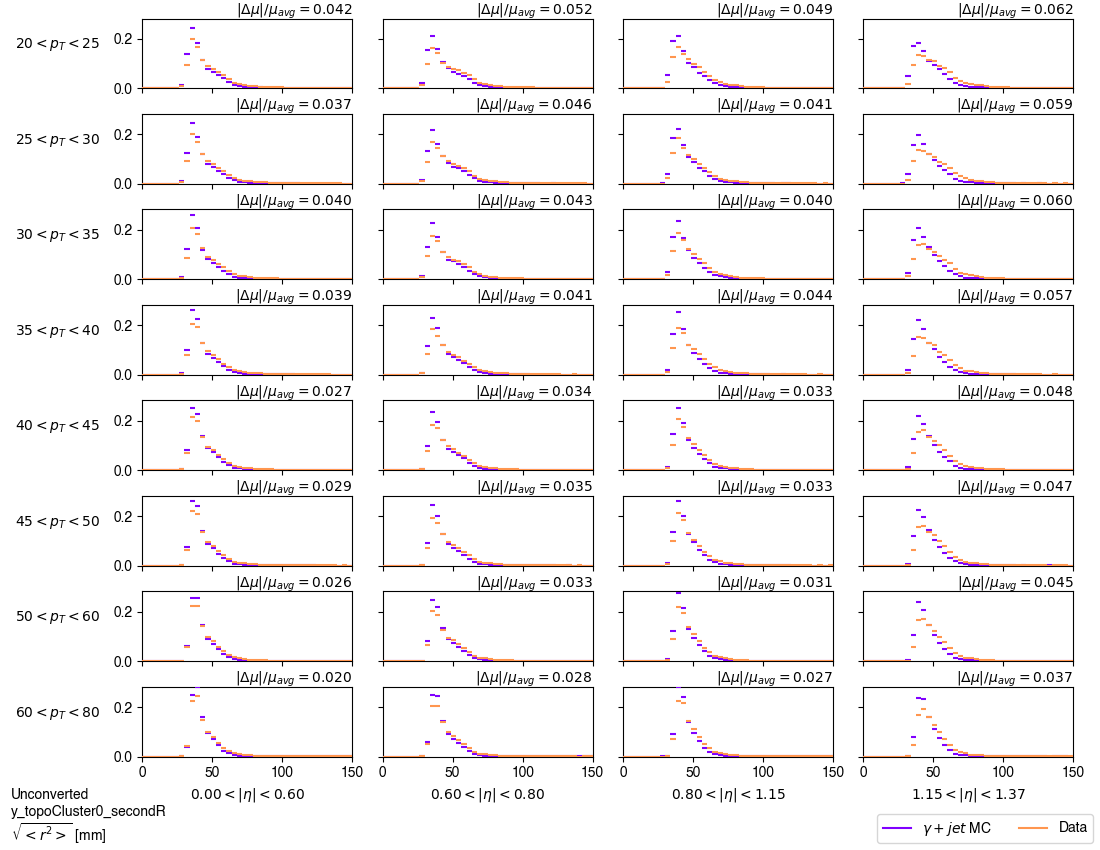
\includegraphics[width=.80\textwidth]{chapters/chapter4_photonID/images/y_topoCluster0_secondR_Unconverted_lowerEta.png}
    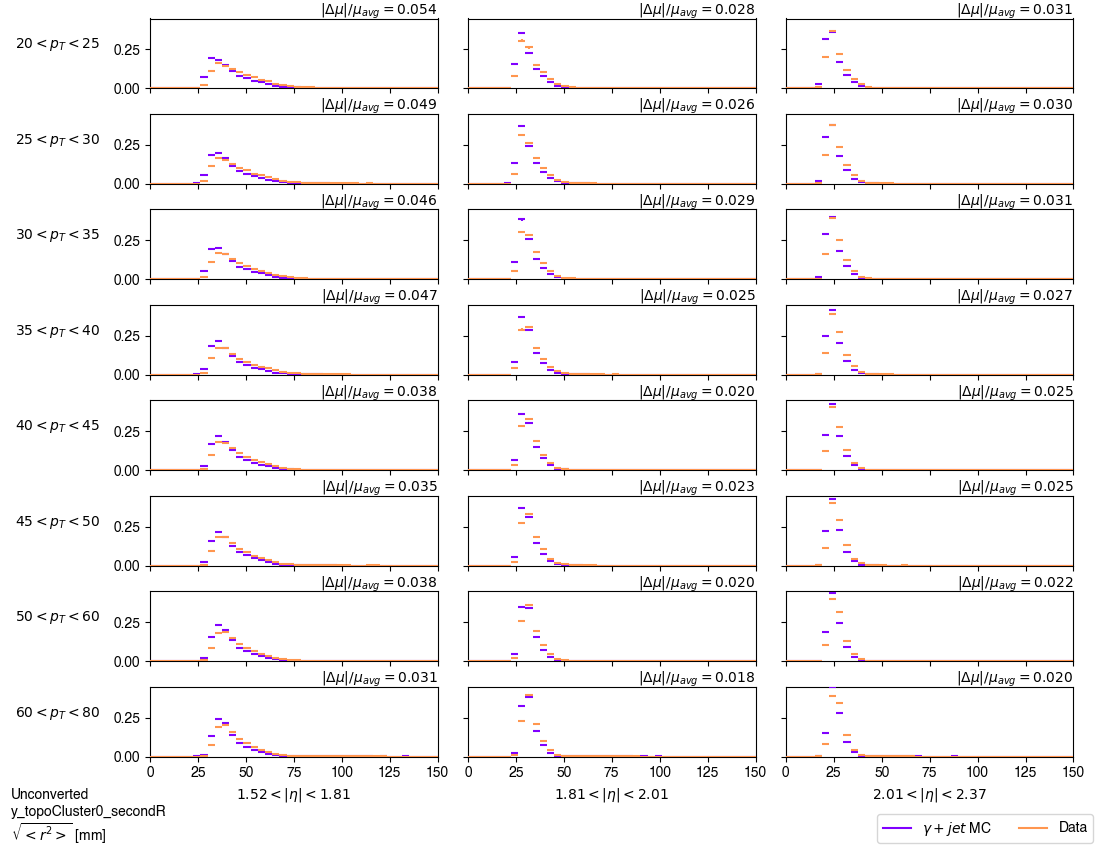
\includegraphics[width=.80\textwidth]{chapters/chapter4_photonID/images/y_topoCluster0_secondR_Unconverted_upperEta.png}
    \caption{Data-MC comparison for the semi-major axis in width ($\sqrt{r^2}$).}
\end{figure}
% TODO: split these figs?

\noindent\textbf{Correlations}\\
\indent Checking the correlations of variables is important for several reasons. First, highly correlated variables do not bring new information, and thus are not useful for adding additional cuts on. Also, it is paramount that any variables that are incorporated in the menu are not correlated to photon isolation. The correlation between these variables and the shower shape variables and isolation working points is shown in Figure \ref{fig:photonid-corrs}. 
%todo: add plots

\begin{figure}[!thp]
    \centering
    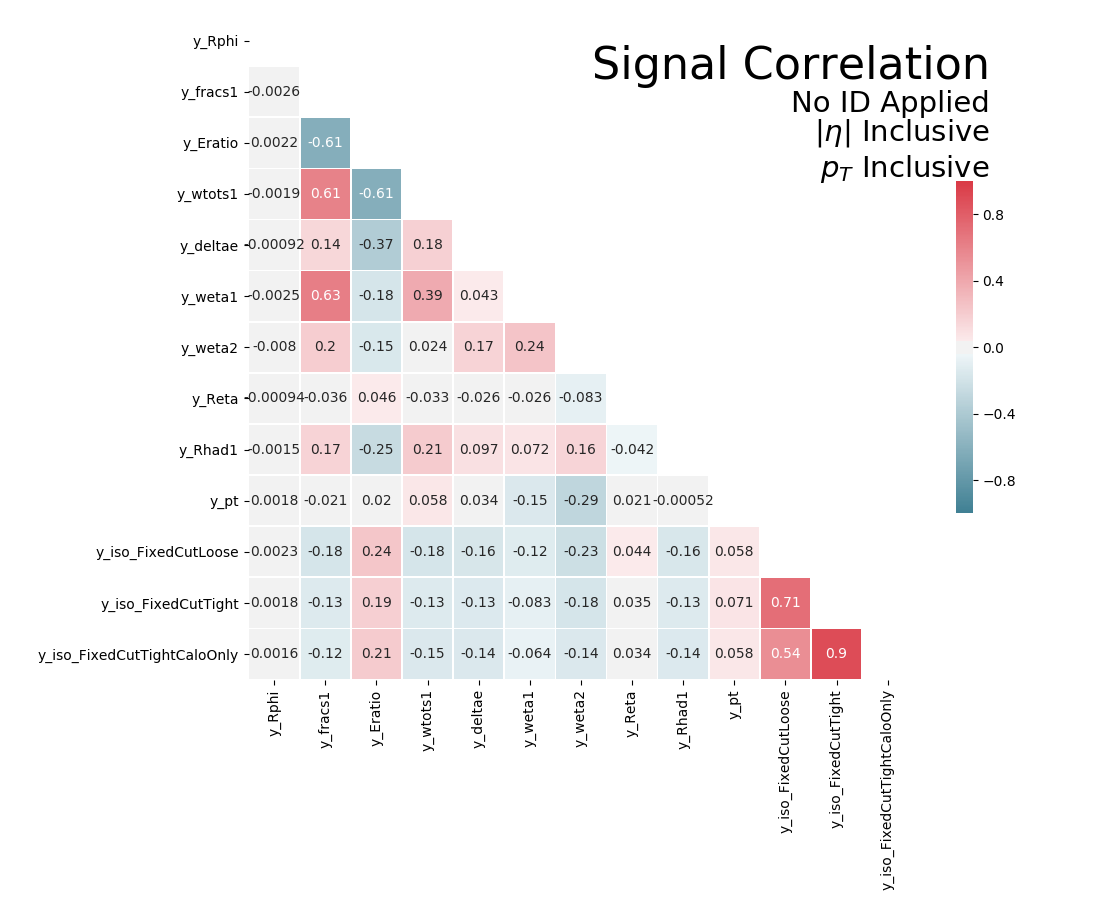
\includegraphics[width=.77\textwidth]{chapters/chapter4_photonID/images/sig_none_corr.png}
    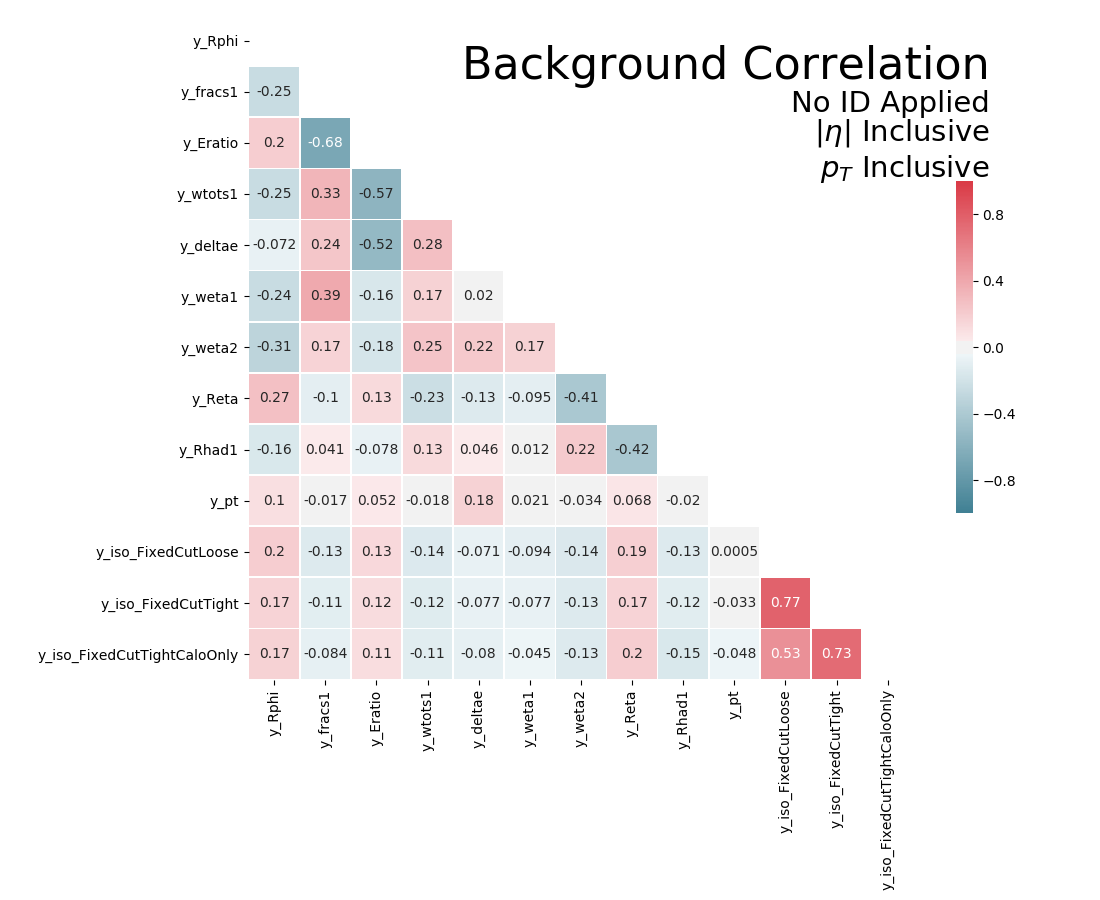
\includegraphics[width=.77\textwidth]{chapters/chapter4_photonID/images/bkg_none_corr.png}
    \caption{Correlation values between the shower shape variables, topological cluster variables, and isolation working points.}
    \label{fig:photonid-corrs}
\end{figure}
% TODO: split these figs?

\subsection{Incorporating into Menu}

The topological cluster variables were added to the existing shower shape variable-based menu. The cut-based approach is reoptimized including the new variables, and new cuts are derived in each $\eta$-\pt bin. To compare improvement across bins, a figure of merit is defined, the improvement in background rejection for the same signal efficiency as the current photon identification menu. In formulaic terms:

\begin{align}
    Z &= \frac{(1-\epsilon_{bkg,i}) - (1-\epsilon_{bkg,0})}{(1-\epsilon_{bkg,0})} = \frac{\epsilon_{bkg,0} - \epsilon_{bkg,i}}{1-\epsilon_{bkg,0}}
    \label{eqn:improvement-metric}
\end{align}

For figure of merit $Z$, and background efficiency $\epsilon_{bkg}$ (thus, background rejection is $(1-\epsilon_{bkg}$), where index $i$ indicates the reoptimized menu, and index $0$ indicates the original menu. This value is calculated bin-wise in $\eta$-\pt and shown in Figure ADD FIG. In principle, adding additional variables to a cut-based method should only improve optimization if the search over possible cut values is exhaustive. However, in several bins, worse performance is found by incorporating new variables. This can be the result of two causes:
\begin{itemize}
    \item In a high dimensional space, such a grid search becomes computationally prohibitive, so a Genetic Algorithm\footnote{The Genetic Algorithm used is a standard method implemented in \texttt{TMVA}, and the details of implementation can be found in Reference \cite{TMVA}.} \cite{genetic-algo} is used to find an approximate solution, and thus increasing dimensionality has the possibility to find local minima, and thus suboptimal solutions.
    \item Statistical fluctuations. As standard, models are trained on an orthogonal subset of events than they are evaluated on, and statistical fluctuations in these samples can influence reported gain, particularly in low stats bins. Figure \ref{fig:photonid-events} shows the number of signal and background events in each $\eta$-\pt bin.
\end{itemize}

\begin{figure}[!thp]
    \centering
    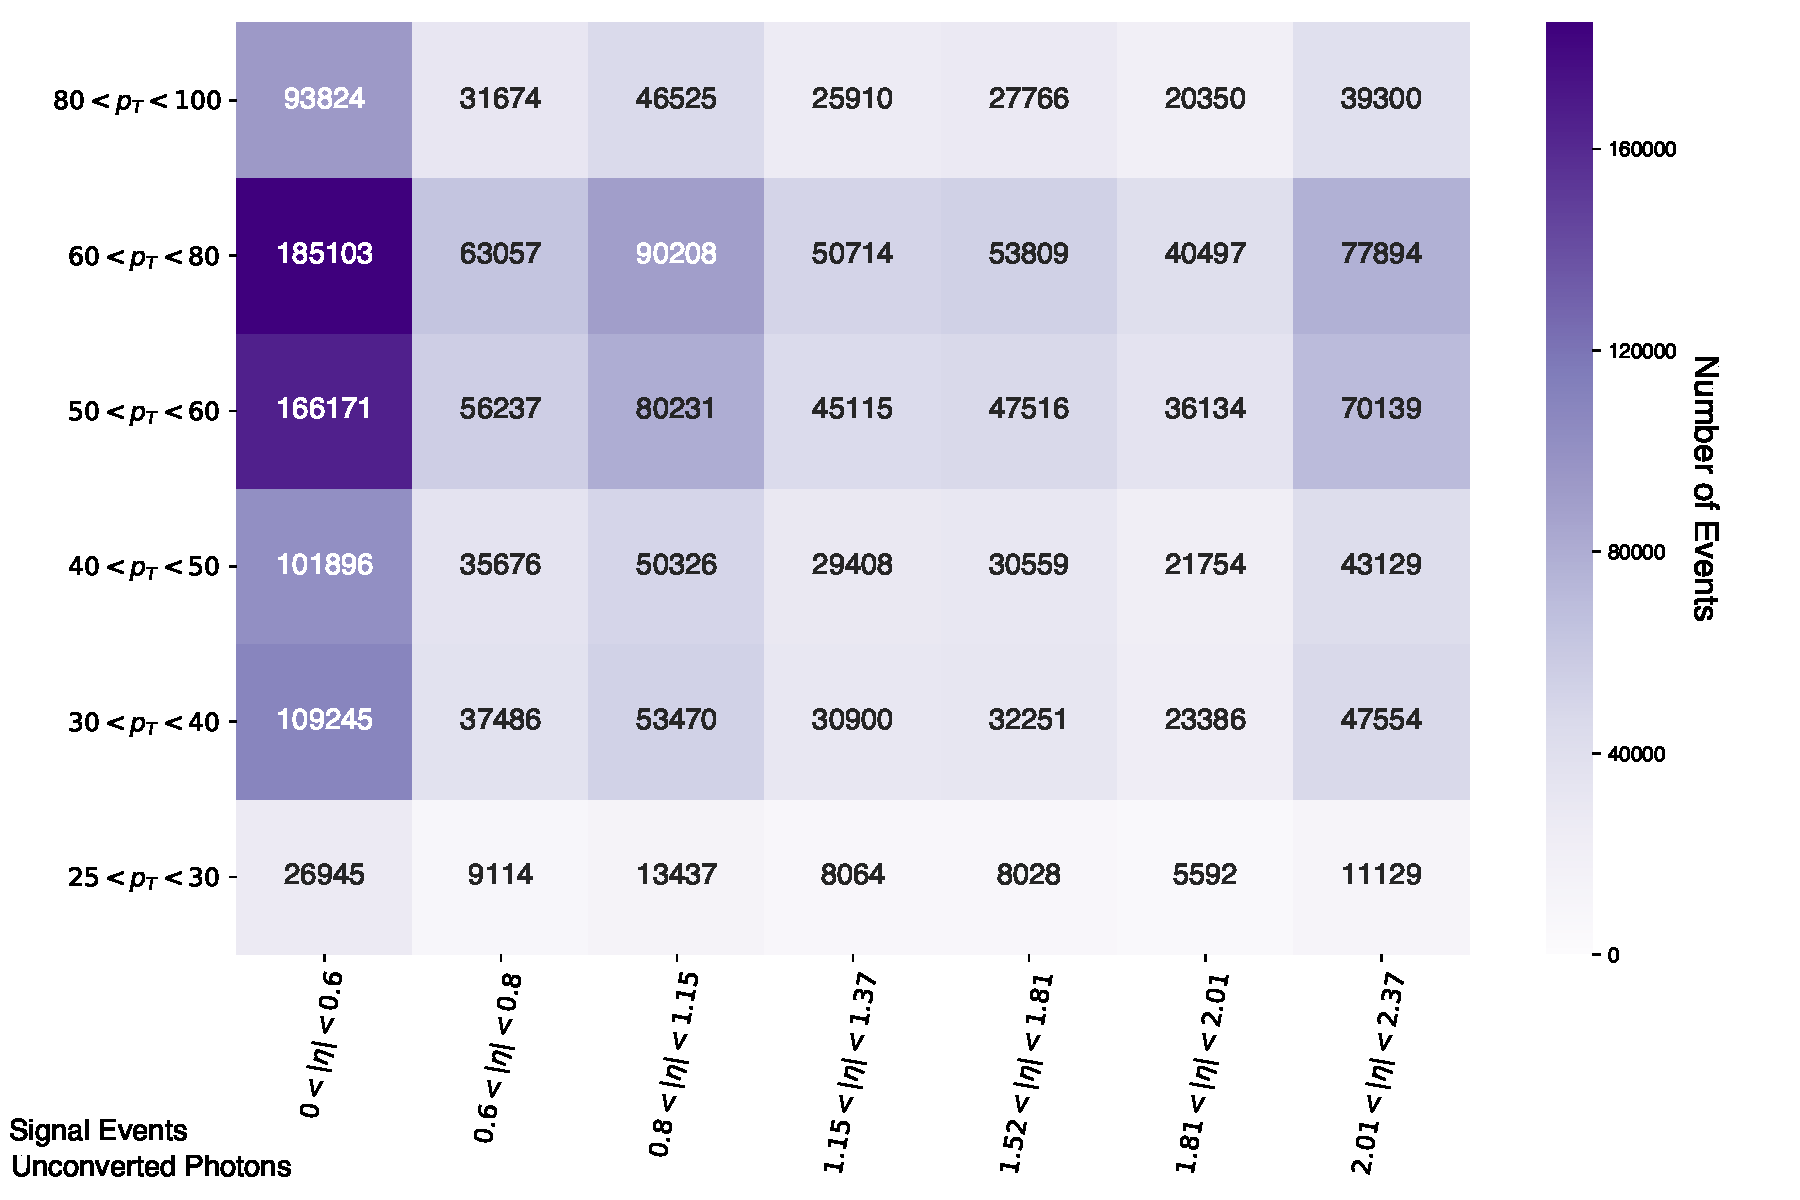
\includegraphics[width=.85\textwidth]{chapters/chapter4_photonID/images/sig_events.pdf}
    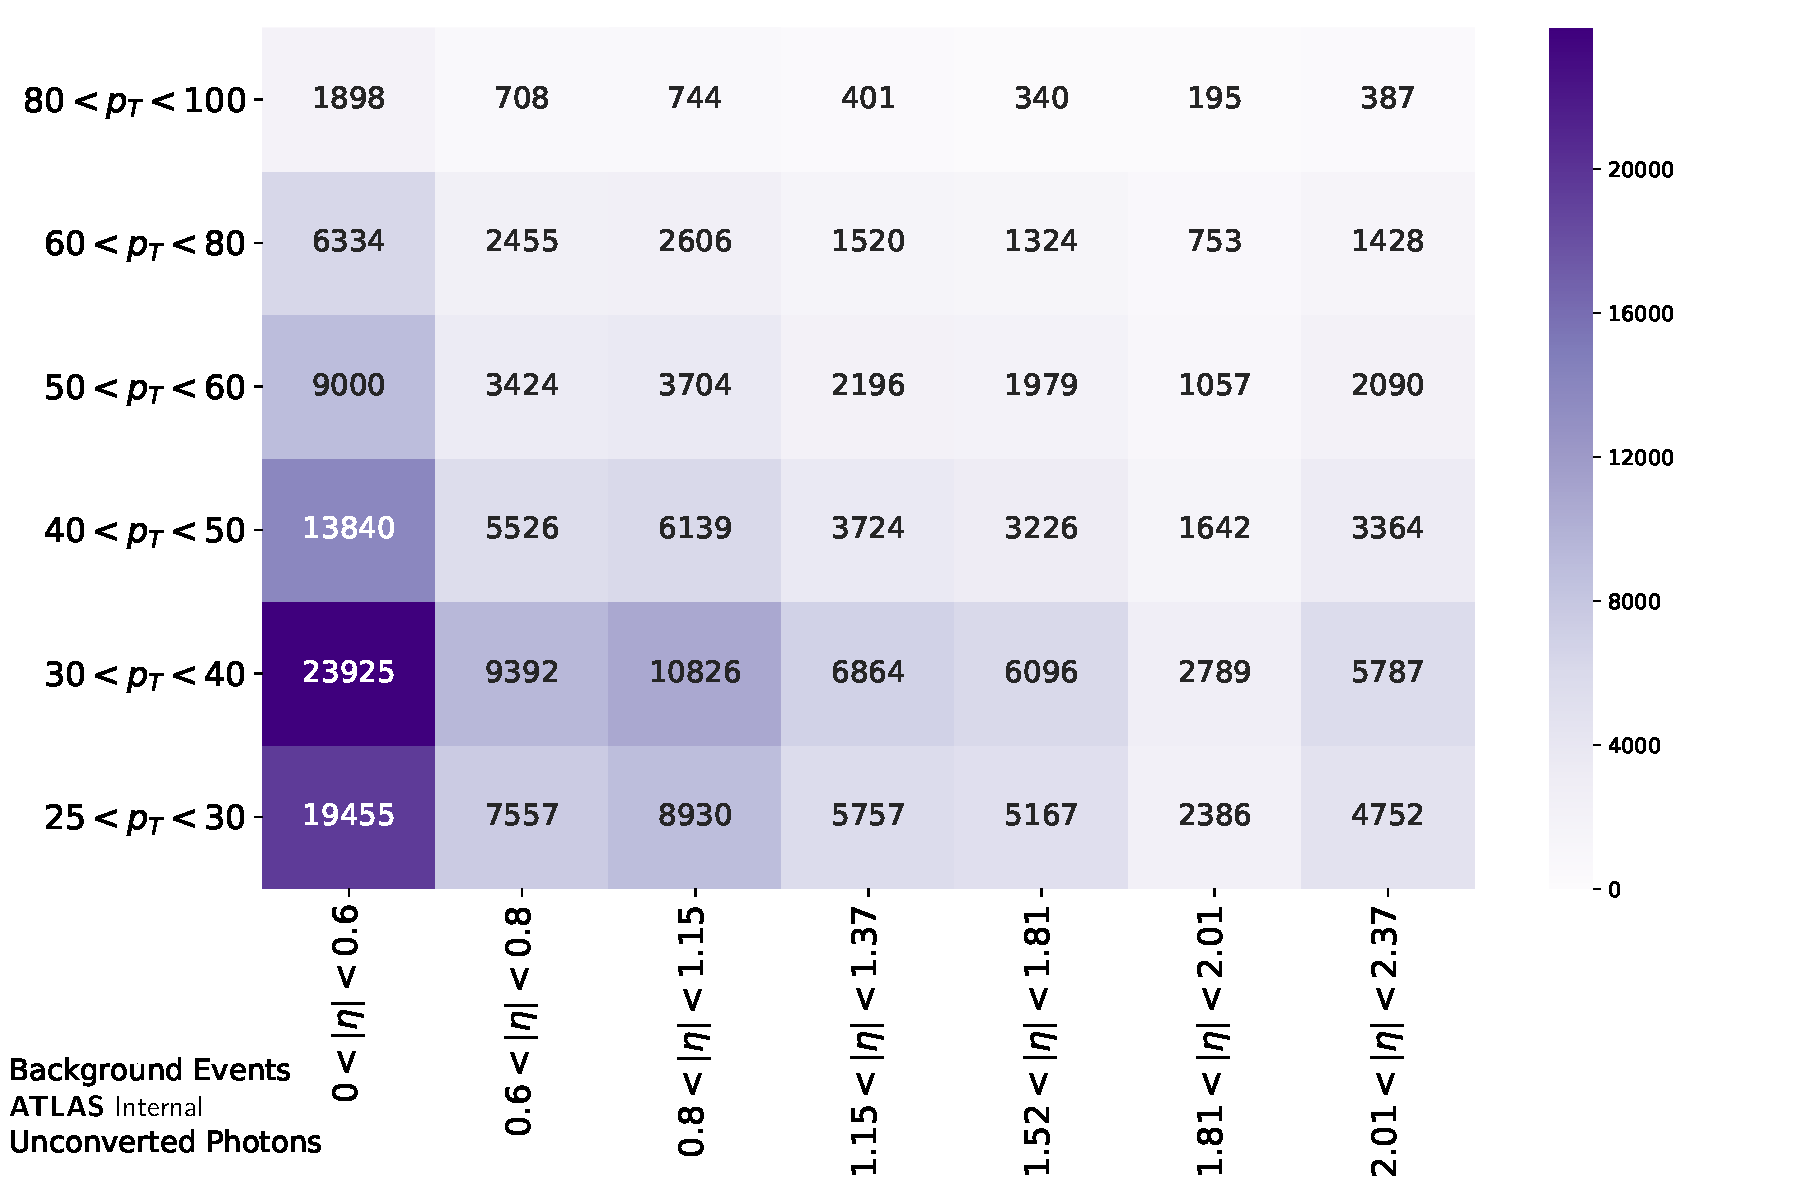
\includegraphics[width=.85\textwidth]{chapters/chapter4_photonID/images/bkg_events.pdf}
    \caption[Number of training events for in each $\eta$-\pt bin for the signal $\gamma$+jets sample, and the background jet fakes sample]{Number of training events for in each $\eta$-\pt bin for the signal $\gamma$+jets sample (top), and the background jet fakes sample (bottom). The preselection described in Section \ref{sec:photon-id-samples} is used.}
    \label{fig:photonid-events}
\end{figure}


\section{Multivariate Analysis Techniques}

The current photon identification working points are defined by a rectangular cuts method. Cut optimization is performed through a 9-dimensional scan over the shower shape variables. In order to better reject background, a multivariate approach to defining these working points has been investigated. These methods are outlined in detail in Appendix \ref{app:MVA}, and the following sections will discuss the improvements brought to photon identification through implementing them.

\subsection{Boosted Decision Tree}

A gradient boosted \gls{BDT} was employed as an alternative classification algorithm. A major problem in training these \glspl{BDT} was the lack of background training statistics when segmenting into $\eta$-\pt bins. To navigate this problem, rather than training an independent model for each $\eta$-\pt bin, \pt inclusive models were trained. As shown in Figure \ref{fig:photonid-corrs}, the input variables have low correlation to \pt, and thus this does not bias the model.


As a baseline, the \gls{BDT} is compared to the cut-based photon identification menu, using the same figure of merit defined in Equation \ref{eqn:improvement-metric}, where the efficiency denoted $i$ represents the \gls{BDT} model, and the efficiency denoted $0$ represents the current cut-based model.


\subsection{Neural Network}

In addition to a \gls{BDT}, a \gls{NN} was studied for photon classification. The \gls{NN} considered the same variables. One was generated 